\documentclass[12pt]{article}
\usepackage[utf8]{inputenc}
\usepackage[T1]{fontenc}
\usepackage{lmodern}
\usepackage{geometry}
\geometry{margin=1in}
\usepackage{amsmath,amssymb}
\usepackage{enumitem}
\usepackage{xcolor}
\usepackage{tikz}

\title{Worksheet: Lecture on SVD (Gilbert Strang, MIT 18.06)}
\author{}
\date{}

\begin{document}
\maketitle

\section*{Before the lecture}
\begin{itemize}
  \item Przypomnij sobie cztery fundamentalne podprzestrzenie.
  \item Sprawdź, czym różni się rzut na kolumny macierzy od rzutu na wiersze.
  \item Zastanów się: jak może wyglądać „najlepsza aproksymacja” macierzy?
\end{itemize}

\section*{Four fundamental subspaces}
Uzupełnij tabelę (własnymi słowami, po polsku lub angielsku):

\bigskip
\begin{tabular}{|c|c|}
\hline
\textbf{Domain $\mathbb{R}^n$} & \textbf{Codomain $\mathbb{R}^m$} \\
\hline
Row space: \hspace{4cm} & Column space: \hspace{4cm} \\
\hline
Nullspace: \hspace{4cm} & Left nullspace: \hspace{4cm} \\
\hline
\end{tabular}

\bigskip
\textit{Pytanie:} Dlaczego row space i nullspace są dopełnieniami ortogonalnymi? 

\section*{Definition of SVD}
Podczas wykładu zapisz własnymi słowami definicję SVD:

\bigskip
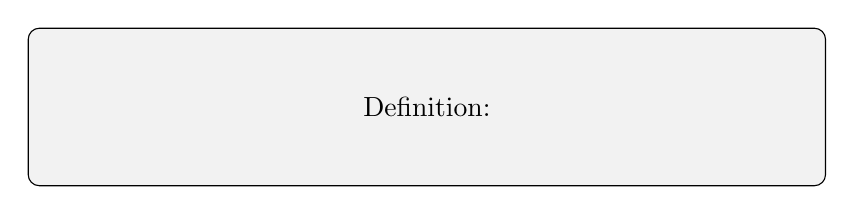
\begin{tikzpicture}
\node[draw,rounded corners,fill=gray!10,minimum width=\textwidth-2cm,minimum height=2cm,anchor=west] (box) at (0,0) {};
\node[align=left] at (box) {Definition:};
\end{tikzpicture}

\bigskip
\textit{Tip:} zwróć uwagę na kolejność: $V^\top$ (obrót/odbicie), $\Sigma$ (skalowanie osi), $U$ (obrót/odbicie).

\section*{Key ideas to notice}
Zatrzymuj wykład i uzupełniaj poniższe miejsca:

\begin{enumerate}[label=\textbf{K\arabic*}.]
  \item Jak Strang łączy SVD z metodą najmniejszych kwadratów?
  \vspace{1cm}
  \item Jak wygląda „geometria SVD” dla okręgu jednostkowego?
  \vspace{1cm}
  \item Co mówi o najlepszej aproksymacji rangą $k$?
  \vspace{1cm}
  \item Jakie przykłady macierzy symetrycznych lub specjalnych pojawiają się w wykładzie?
  \vspace{1cm}
\end{enumerate}

\section*{Discussion questions}
\begin{itemize}
  \item Jak SVD łączy się z fundamentalnymi podprzestrzeniami?
  \item Dlaczego pseudoodwrotność można najprościej zapisać przez SVD?
  \item Jak myślisz: czemu SVD jest ważniejsze praktycznie niż rozkład na wartości własne?
\end{itemize}

\section*{English Corner}
Hasła, które padną na wykładzie – uzupełnij własnym tłumaczeniem:
\begin{itemize}
  \item singular values
  \item left/right singular vectors
  \item least squares
  \item projection
  \item best rank-$k$ approximation
\end{itemize}

\bigskip
\textbf{Task:} Wybierz jedno hasło i napisz własne zdanie po angielsku, używając go poprawnie.

\end{document}
